\documentclass[oneside]{book}

% Load the VUB package.
% This has many options, please read the documentation at
% https://gitlab.com/rubdos/texlive-vub
\usepackage{vub}

%href package to make references clickable.
\usepackage{hyperref}
\hypersetup{
    colorlinks,
    citecolor=black,
    filecolor=black,
    linkcolor=black,
    urlcolor=black
}

% Better math equations
\usepackage{amsmath}

% Some highly suggested packages, please read their manuals.
\usepackage{cleveref}
\usepackage[natbib,style=apa]{biblatex}
\addbibresource{../bibliography.bib}
\usepackage{listings}
\usepackage{wrapfig}


%smaller spacing
\usepackage{titlesec}
\titlespacing*\section{0pt}{12pt plus 4pt minus 2pt}{0pt plus 2pt minus 2pt}
\titlespacing*\subsection{0pt}{12pt plus 4pt minus 2pt}{0pt plus 2pt minus 2pt}
\titlespacing*\subsubsection{0pt}{12pt plus 4pt minus 2pt}{0pt plus 2pt minus 2pt}

%space between paragraph and indent all
\setlength{\parskip}{1em}
%\usepackage{indentfirst}

% algorithms
\usepackage{algpseudocode}
\usepackage{algorithm}

%quotes
\usepackage{epigraph}

%space between bib entries
\setlength\bibitemsep{2\itemsep}

%images settings
\graphicspath{ {./images/} }
\usepackage{graphicx,caption}
\usepackage{float}
\usepackage{rotating}
\usepackage{tikz}

% subfigures
\usepackage{subcaption}

% remove chapter text
\usepackage{titlesec}

\titleformat{\chapter}[display]
  {\normalfont\huge\bfseries}{}{0pt}{\Huge}
\titlespacing*{\chapter}
  {0pt}{0pt}{15pt}

%START title
\title{Self-organization in vowel systems from small communities}
\subtitle{Extending de Boer 2000 - EoS project}
\author{Lennert Bontinck}
\date{January, 2021-2022}
\promotors{Student number: 0568702}
\faculty{Computer Science: AI}
\begin{document}
\frontmatter
\maketitle
%END title


%TOC
\tableofcontents
\mainmatter

%START MAIN
\chapter{Project goal and supplied code}
\label{ch:general_remarks}

During the Evolution of Speech course taught at the VUB in 2021-2022 we, Computer Science students, were introduced to this multidisciplinary field by reviewing multiple important papers of the field.
As the course was taught by Bart de Boer, who has an Oxford  University Press published book on the origins of vowel systems and many papers in the field, we also reviewed some of de Boer's papers (\cite{deBoerBook, deBoer2000, deBoer2010, deBoer2018}).
As a Computer Science student with limited linguistic knowledge, papers from de Boer using Agent-Based Modelling (ABM) techniques for studying phenomena in the field were found the most interesting (\cite{deBoer2000, deBoer2010}).
Because of this, we opted to extend upon \citet{deBoer2000}.
The exact project goal and an overview of the supplied code are given in further detail here.

%------------------------------------

\section{Project goal}
\label{sec:general_remarks_why}
It was chosen to re-implement and extend the paper on self-organization in vowel systems by \citet{deBoer2000} for this project.
Whilst the original C++ source code of \citet{deBoer2000} was provided to us, his students, it was dated and not so well documented.
This was to be expected as the code was not originally meant for distribution.
To further ground our understanding of the paper and make extensions on this work easier, we have chosen to do a re-implementation in Python.
The written code is well documented, easily extendable and most importantly, publicly available under the GPL V3 license \citep{gplv3, github_project}.
This enables readers to not only easily reproduce the results of \citet{deBoer2000} and the extensions provided here but also gives them a great basis for future projects.
The latter was something we felt was lacking and feel is an important contribution of this work.
We also addressed some of the \textit{ad hoc} decisions in the original version.
To be more precise, this report provides an alternative way of converting to the bark scale and determining the effective second formant of a produced sound.
This was found to not influence the results, as is further discussed in chapter \ref{ch:improving_de_boer}.

In the original version of the imitation game proposed by \citet{deBoer2000}, agent pairs are picked at random.
Whilst this is an understandable simplification for his work, it made us wonder if the findings hold for more complex structures.
Initially, it was considered to use scale-free networks, as we thought this would better represent a human network.
However, the actual realism of scale-free networks is debated and one of our colleagues wanted to go this route already \citep{scalefreebad}.
Because of this, we opted to model a small community consisting of agents with different roles and influences.
These agents and their roles evolve over time to eventually be replaced with new agents.
It is thus a more dynamic and varying setting than the one used by \citet{deBoer2000}.
This is done to further ground the initial hypothesis by de Boer, namely: "The structure of vowel systems is determined by self-organization in a population under constraints of perception and production." - \citet{deBoer2000}.

%------------------------------------
\section{Important files}
\label{sec:general_remarks_files}

Accompanied by this report is a copy of the GitHub repository created for this project \citep{github_project}.
It includes all files needed to reproduce the experiments, including saved versions of the games used for figures and statistics in this report.
An overview of the most important files is given below:
\begin{itemize}
    \item \texttt{README.md}
    \begin{itemize}
        \item General information of the GitHub repository with hyperlinks to important files and documentation. 
    \end{itemize}
    \item \texttt{code-output}
    \begin{itemize}
        \item All figures generated by the provided code, some of which are used in this report.
    \end{itemize}
    \item \texttt{code/notebooks}
    \begin{itemize}
        \item Jupyter notebooks and plain py files going over different aspects of the code for this project.
        \item \texttt{1\_implementing\_de\_boer\_2000.ipynb}: step by step re-implementation of code by \citet{deBoer2000}.
        \item \texttt{imitationGameClasses.py}: all classes needed to play imitation games as specified by \citet{deBoer2000}.
        \item \texttt{2\_recreating\_de\_boer\_2000.ipynb}: step by step re-collection of results by \citet{deBoer2000}.
        \item \texttt{3\_alternative\_bark\_experiments.ipynb}: step by step re-collection of results by \citet{deBoer2000} using a less ad hoc variant of the bark converter and effective second formant weighting function.
        \item \texttt{4\_adding\_small\_communities.ipynb}: step by step implementation of the community based imitation games (extension).
        \item \texttt{communityImitationGameClasses.py}: all classes needed to play the community based imitation games.
        \item \texttt{5\_evaluating\_small\_communities.ipynb}: evaluation of the community based imitation games.
    \end{itemize}
    \item \texttt{code/html-exports} and \texttt{documentation/installation}
    \begin{itemize}
        \item HTML export of the above discussed Jupyter notebooks, ideal for those who want to view the notebooks without installing the Anaconda environment.
        \item Install instructions for the used Anaconda environment of this project (macOS and Ubuntu).
    \end{itemize}
\end{itemize}
\chapter{Relevant literature}
\label{ch:literature}

In this chapter, a summary of the most important aspects of \citet{deBoer2000} is given.
We also discuss some literature on network structures in ABMs to further defend why we think our extension is a useful one.

%------------------------------------

\section{Summary of de Boer (2000)}
\label{sec:literature_db2000}

It was seen from previous work, such as that by \citet{landl}, that functional properties give rise to human-like vowel systems.
Such findings are often found through direct optimisation, in the case of \citep{landl} this is by doing a minimisation on the potential energy to find that optimising for acoustic difference gives rise to realistic vowel systems.
However, whilst such findings are great, they give rise to another question, \textit{how} does this optimisation take place.
This \textit{how} question is one that \citep{deBoer2000} tries to understand by studying an ABM playing imitation games.
This paper of \citet{deBoer2000} is inspired by his PhD thesis, which is longer and more detailed \citep{deBoerFull}.
If the ABM, which makes use of simple self-organised agents, gives rise to human-like vowel systems, it \textit{could} be possible that self-organisation played an important role in the evolution of speech.
This could part is important, as ABMs can't directly prove a hypothesis.

The ABM described by \citet{deBoer2000} consists of agents who play imitation games.
These imitation games consist of two randomly picked agents where one is the \textit{speaker} and the other is the \textit{imitator}.
The speaker says a random sound from his \textit{sound repetoire}.
The imitator replies with one of his known sounds that lies closest to the \textit{perceived} one.
The speaker then communicates a \textit{non-verbal} signal to either confirm or reject the imitation to be correct.
A correct imitation is one where the perceived sound is closest to the initially produced sound for the speaker.
The imitator uses this information to update his sound repertoire.
The sound repertoires of agents are non-fixed and initially empty.
From this description it becomes clear an agent should have three important skills: a sound \textit{production}, \textit{perception}, and \textit{storing} mechanism.
Besides this, the agent should also be able to \textit{learn} from the non-verbal signals.
Chapter \ref{ch:reimplementing} re-implements this ABM, where it is described in more detail how these different components work and some of the \textit{ad hoc} decisions made by \citet{deBoer2000} to make it work.

Chapter \ref{ch:reimplementing} goes into more detail on the metrics used to evaluate the findings of this ABM.
In that chapter, the found evaluation metrics are also replicated.
From these found results, \citet{deBoer2000} concludes that self-organization can explain properties found in human vowel systems.
He states that one should not study a vowel system by its individual vowels (as done by \cite{chomsky}) or as a whole \citep{landl} but rather concerning the population it is used in.
This work by \citet{deBoer2000} remains one of his most cited works and has proven to be influential in the field.
Because of this, we found it fit to re-implement it so that newcomers can get a grasp on experiments in the field and to further defend the findings by \citet{deBoer2000}.







%------------------------------------

\section{Importance of network structure for emergence}
\label{sec:literature_emergence}

The extension to the above discussed ABM provided with this report is one on the network structure used.
As discussed, the pair of agents to play an imitation game each iteration are chosen at random in the implementation of \citet{deBoer2000}.
Given enough iterations, this will evolve from a random network to a fully connected network.
This contradicts with human networks where a certain hierarchy exists and not every person will adopt his speech to another person.
For example, a professor in the English language would not adopt his sound repertoire to that of a newborn.
More importantly, the results of ABMs have been shown to depend heavily on the underlying communication network used, whether they are used in linguistic applications or not \citep{network1, network2, network3}.

To model human communities, scale-free networks are often used.
Scale-free networks are networks where the degree distribution of nodes follows a power law.
A preferential attachment like property in human psychology is often given as a reason that these networks are well representative of a human social network \citet{scalefreegood}.
However, it is often debated whether such scale-free networks appear as often in nature as it is claimed to by some \citep{scalefreebad}.

Another commonly used network is a \textit{small-world} network.
An overview of these three network structures is given in Figure \ref{fig:network_structures}.
Many other network structures exist as it is an important topic of graph theory.
We believe a network that lies between small-world and scale-free networks is a good fit to represent early human communities.
Hence, such a directed and weighted network is presented in chapter \ref{ch:extension}.


\begin{figure}[H]
    \centering
    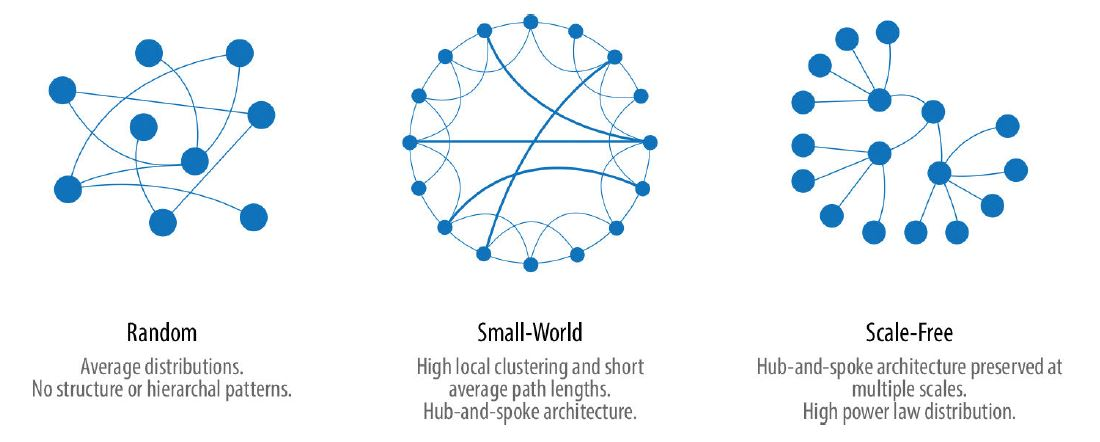
\includegraphics[width=\linewidth]{images/literature/network_structures.jpeg}
    \captionsetup{width=0.9\linewidth}
    \captionsetup{justification=centering}
    \caption{Random, small-world and scale-free networks. Figure by \citet{graphsfigure}.}
    \label{fig:network_structures}
\end{figure}


\chapter{Re-implementing de Boer (2000)}
\label{ch:reimplementing}
% beter gebruik classes en doc
% formules van ons vergelijken met die van de boer want soms anders in paper en code
% cleaner afgaan van mogelijke shift
% semi random add ipv random zoals gezegd
% equal van vowels beter bespreken

The original C++ source code of \citet{deBoer2000} was provided to us, de Boer's students.
However, this code was dated and not meant for distribution, which made it difficult to be used or extended upon.
Because we saw the value in a well documented and easy to extend implementation of this project, we decided to fully re-implement it in Python.
This was done incrementally, with each step described in \texttt{1\_implementing\_de\_boer\_2000.ipynb}.
The working of the code was validated by reproducing the results of the experiments by \citet{deBoer2000} in \texttt{2\_recreating\_de\_boer\_2000.ipynb}.
This chapter will summarise the development and findings of these two Jupyter notebooks.
We stress that all of the discussed code in what follows is either derived from textual description in \citet{deBoer2000} or the provided C++ code.

%------------------------------------

\section{Producing sounds}
\label{sec:reimplementing_producing}

\citet{deBoer2000} system consists of agents who can produce, perceive, and remember speech sounds in a human-like way.
The most important component for producing sounds in a human-like manner is the articulatory synthesizer.
This synthesizer takes as input three vowel parameters: the tongue position ($p$), the tongue height ($h$) and the lip rounding ($r$).
The outputs of the synthesizer are the first four formant frequencies of the corresponding vowel: $F_1$ to $F_4$ expressed in $Hz$.
The conversion between input and output happens based on the synthesizer equations given by \citet{deBoer2000}, table 2.
\Citet{deBoer2000} used interpolation from known data to create these equations.
We used these known points for validating our $F_1$ to $F_4$ conversions from the $p$, $h$ and $r$ input and found them to match perfectly with the given data.

From the above-described synthesizer equations, we can make the \texttt{Synthesizer} class.
To represent input and output formally, we make use of two helper classes: \texttt{Utterance} and \texttt{Phoneme}.
The former stores an utterance consisting of the four formants $F_1$ to $F_4$.
This is the output of the \texttt{synthesise} function.
A phoneme is used as input for the same function and stores the $p$, $h$ and $r$ parameters.
Two types of noise can be assigned to a \texttt{Synthesizer} object.
The \texttt{max\_noise\_agent} and the \texttt{max\_noise\_ambient}.
The agent noise is applied to the phoneme before utterance creation (Equation \ref{eq:reimplementing_noise_agent}), the ambient noise is applied to the utterance after creation.
The applied noise, $\lambda$, is uniformly picked from: $\frac{-\psi}{2} \leq \lambda \leq \frac{\psi}{2}$, with $\psi$ being the provided parameter.
$\psi$ is one of many important parameters.
In the experiments by \citet{deBoer2000}, only the ambient noise is used.

\begin{equation}
F^{agent}_{i}(p, h, r) = F_{i}(p + \lambda, h + \lambda, r + \lambda)
\label{eq:reimplementing_noise_agent}
\end{equation}

\begin{equation}
F^{ambient}_{i} = F_{i} * (1 + \lambda)
\label{eq:reimplementing_noise_ambient}
\end{equation}

%------------------------------------
\section{Perceiving sounds}
\label{sec:reimplementing_perceive}

With the \texttt{Synthesizer} and helper classes in place, an agent can produce a signal that represents sound in a human-like manner.
For an agent to perceive these signals in a human-like manner, the \texttt{Bark Operator} class is created.
This class is responsible for working with utterances.
Remember that utterances were the first four formants of a generated sound, in Hertz.
As the name of this class implies, the Bark scale is used by this class and is differing from the previously used Hertz scale. 
It represents frequencies in a manner that is closer to human perception.
It goes from the four formant representation in Hertz to a two formant representation in Bark consisting of the first formant and the \textit{effective second-formant} ($F'_2$).

We took the conversion formulae and calculation formula for the effective second formant straight from \citet{deBoer2000}.
The conversion from Hertz to Bark and back used by \citet{deBoer2000} is again interpolated from data.
It is also admitted by \citet{deBoer2000} that his calculations for determining ($F'_2$) are a bit ad hoc.
The critical distance used for calculating ($F'_2$) can be provided as an optional argument.
Because of the interpolated conversion and ad hoc ($F'_2$) calculations, we have also foreseen an \texttt{alternative\_bark\_conversion} parameter.
If set to \texttt{True}, the Bark operator will use alternative methods for both of these functions.
This is further discussed in section \ref{sec:reimplementing_better}.

Having our Bark space configured, we can implement a distance measure between utterances as specified in Equation \ref{eq:reimplementing_distance}.
This distance measure can be used as a way for the agent to determine the closest sound in his repertoire to the one it heard.
This must happen in the Bark space as equal distances in bark correspond to roughly equal human-perceptual distances of sound.
This is not the case for Hertz, as humans have a harder time differentiating higher frequencies.
With this human-like distance measure, agents can now perceive sounds and compare them with their known sounds.
This $\lambda$ is again an important parameter for the simulations.
It is set to $0.3$ for all experiments in the project unless specified differently.
This value is seen as realistic by \citet{Schwartz1997, deBoer2000, vallee1994, 1985book}.

\begin{equation}
D = \sqrt{ ( F^a_1 - F^b_1 ) ^2 + \lambda ( F'^a_2 - F'^b_2 )^2 }
\label{eq:reimplementing_distance}
\end{equation}

%------------------------------------
\section{Representing agents}
\label{sec:reimplementing_agents}

The \texttt{Agent} class makes use of all previously discussed classes as well as the \texttt{Sound} helper class.
The \texttt{Agent} class takes a synthesizer and Bark operator as arguments for initialising.
It also has over ten optional parameters one of which is a logging capability handy for debugging purposes.
The \texttt{Sound} class is used to store a known sound of an agent.
It consists of the phoneme, utterance, usage count and success count of the sound.
The utterance of this sound is determined by synthesising the provided phoneme in a noiseless environment.

To discuss the functions of an agent, it is easiest to present a typical imitation game flow.
Algorithm \ref{alg:say_something} shows the actions performed by a randomly picked agent who starts an imitation game.
If the agent known sound repertoire is empty a completely random vowel is inserted by picking random values between $0$ and $1$ for the Phoneme parameters.
A different randomly picked agent plays the role of imitator and response to the heard utterance using the process shown in Algorithm \ref{alg:imitate_sound}.
If the imitator's known sounds repertoire is empty, it will add a \textit{similar sound} to the one it heard.
It does this by checking eight \textit{corner} sounds it can produce and picking the one which is closest in distance.
Afterwards it improves this sound further by using its \texttt{improve\_sound} function for the agent specific amount of times (\texttt{max\_similar\_sound\_loops} parameter).
The \texttt{improve\_sound} function tries all possible permutation's of the phoneme parameters by either keeping the value or adding/substracting the agent specific step size (\texttt{phoneme\_step\_size} parameter).

%-----------------------------------------------------

\begin{algorithm}[hbt!]
\caption{The say\_something function of an imitation game initiator agent}\label{alg:say_something}
\begin{algorithmic}
\If{No known sounds}
    \State Add random sound to known sounds
\EndIf

\State $S \gets$ random known sound
\State Update usage count of $S$
\State Remember chose of $S$
\State Return utterance of $S$ using own bark operator


\end{algorithmic}
\end{algorithm}

%-----------------------------------------------------

\begin{algorithm}[hbt!]
\caption{The imitate\_sound function of an imitator}\label{alg:imitate_sound}
\begin{algorithmic}
\Require $U_{in}$: the heard utterance
\If{No known sounds}
    \State Add similar sound for $U_{in}$ to known sounds
\EndIf

\State Remember $U_{in}$
\State Find closest known sounds $S$ to heard utterance
\State Update usage count of $S$
\State Remember chose of $S$
\State Return utterance of $S$ using own bark operator


\end{algorithmic}
\end{algorithm}

%-----------------------------------------------------

In the second phase of the game, the initiator validates the imitation it hears in a non-verbal manner.
This process is shown in Algorithm \ref{alg:validate_imitation}.
The agent validates if the closest known sound to the heard imitation utterance is the sound he used to start the game.
He also communicates this to the imitating agent in a non-verbal manner.
He updates the success count accordingly and prepares himself for the next round.
The process of preparing for a new round is given in Algorithm \ref{alg:prepare_new}.
This consists of resetting the game variables such as the $last\_spoken\_sound$ variable.
The agent then updates its count of games played, ads well as the success and imitator/initiator count respectively.
Based on the agent specific \texttt{cleanup\_prob}, \texttt{new\_sound\_prob} and \texttt{merge\_prob} the agent will potentially remove bad sounds, add a semi-random new sound or merge similar sounds.
A sound is thus removed periodically if it's success rate is below the agent specific \texttt{sound\_threshold\_agent} and used at least \texttt{sound\_minimum\_tries}, which is also agent specific.
A sound is also added semi-randomly on a periodic basis.
We call this process semi-random as multiple random vowels will be tried based on the agent specific \texttt{max\_semi\_random\_loop}, and the sound that had the greatest summed distance will be used as new sound.
Finally, similar sounds are also merged on a periodic basis.
The agent does this by validating if both the utterance or phonemes don't lie too close.
Phonemes lie too close if their parameters differ less then 0.17 in total.
Utterance are too close if they can't be distinguished taking into account the noise of the environment.
Both of these calculations are taken from the code provided by \citet{deBoer2000}.


%-----------------------------------------------------

\begin{algorithm}[hbt!]
\caption{The validate\_imitation function of an initiator}\label{alg:validate_imitation}
\begin{algorithmic}
\Require $U_{in}$: the heard imitation utterance

\State Retrieve last spoken sound $S$
\State Find closest known sounds $S'$ to heard utterance
\State $success \gets$ $S = S'$ ?
\If{$success$}
    \State Update success count of $S$
\EndIf

\State Prepare for new game
\State Return $success$
\end{algorithmic}
\end{algorithm}

%-----------------------------------------------------

\begin{algorithm}[hbt!]
\caption{The prepare\_for\_new\_game function of an agent}\label{alg:prepare_new}
\begin{algorithmic}
\Require $imitator$: whether or not the agent was an imitator in the played game
\Require $success$: whether or not the played game was a success

\State Update agent games count
\If{$success$}
    \State Update agent success count
\EndIf

\If{$imitator$}
    \State Update agent imitator count
\Else
    \State Update agent initiator count
\EndIf

\State Remove bad sounds per agent specific odd
\State Merge similar sounds per agent specific odd
\State Add semi-random sound per agent specific odd

\State Reset game variables

\end{algorithmic}
\end{algorithm}

%-----------------------------------------------------
\newpage
To end a game cycle, the imitator agent will process the non-verbal imitation success communication.
It does using the process described in Algorithm \ref{alg:non_verbal}.
If the imitation was successful the agent will use the previously described \texttt{improve\_sound} function once to make the spoken sound better match the heard utterance.
If the imitation was not successful and the used sound has a success ratio lower then the agent specific \texttt{sound\_threshold\_game}, the sound is also improved as described before.
However, if the success ratio of the sound is above this threshold it is assumed that the spoken sound is a correct imitation of other sounds in the network and thus a similar sound is added to the one heard as reaction.
The process of adding this similar sound is identical as described when the sound repertoire of an imitator was empty.


\begin{algorithm}[hbt!]
\caption{The process\_non\_verbal\_imitation\_confirmation function of an imitator}\label{alg:non_verbal}
\begin{algorithmic}
\Require $success$: whether or not the imitation was a success


\State Update agent games count
\If{$success$}
    \State Update agent success count
    \State Improve used sound to better match heard utterance
\ElsIf{Low success ratio of spoken sound}
    \State Improve used sound to better match heard utterance
\Else
    \State Add a similar sound to the heard utterance
\EndIf

\State Remove bad sounds per agent specific odd
\State Merge similar sounds per agent specific odd
\State Add semi-random sound per agent specific odd

\State Reset game variables

\end{algorithmic}
\end{algorithm}

%------------------------------------
\section{Playing and analysing games}
\label{sec:reimplementing_game_engine}
% Game engine en Game State kort beschrijven 
TODO

%------------------------------------

\section{Improving de Boer (2000)}
\label{sec:reimplementing_better}
% BV die dingen dat ad-hoc waren en jij beter gemaakt hebt 
% andere bark gebruikt (conversion en effective second formant)
% Mss betere weighting factors bezien
TODO
\chapter{Resolving some ad hoc decisions from de Boer (2000)}
\label{ch:improving_de_boer}

In the previous chapter, we discussed the re-implementation of the imitation games as proposed by \citet{deBoer2000}.
We mentioned that both the vocal synthesizer and bark conversion were interpolated from publicly available data.
The calculations for determining effective second formant weight ($F'_2$) were found rather ad hoc and definitions varied between the paper and the available code.

We think the design decision to model the vocal tract from interpolated data is understandable in this context.
Not only is it faster than modelling a more complex synthesizer, but the fact that 18 different vowels were used for the interpolation makes it a reasonable approximation.
Especially when considering far fewer sounds were learned on average by the agents due to the limited acoustic space, we think the interpolated vocal tract doesn't impose a conflict for the study.
However, the interpolated bark conversion and calculations for $F'_2$ were something we think could influence the results.
For this reason, this chapter will go into detail on how we tested variants for these calculations using the alternative bark operator.

%------------------------------------

\section{Alternative bark conversion}
\label{sec:alternative_bark_conversion}

When discussing the \texttt{Bark Operator} class in section \ref{sec:reimplementing_perceive} we mentioned the inclusion of the optional \texttt{alternative\_bark\_conversion} parameter.
When this parameter is set to \texttt{True} both the conversion from Hertz to bark and back as well as the $F'_2$ calculations will differ from those described in Equation \ref{eq:bark_conversion_de_boer} and \ref{eq:f2_conversion_de_boer} respectively.

It was found that there is no single definition for the bark scale.
After comparing multiple variants we decided to settle for the bark conversion used by MatLab\footnote{\url{https://nl.mathworks.com/help/audio/ref/hz2bark.html}}.
The conversion from Hertz to bark is given in Equation \ref{eq:bark_conversion_matlab}.
The inverse can analytically be derived and was tested in the \texttt{2\_recreating\_de\_boer\_2000.ipynb} notebook.

\begin{equation}
\begin{aligned}
  \texttt{intermediate} &= \frac{26.81 * Hz}{1960 + Hz} - 0.53 \\
  bark &= 
    \begin{cases}
      \texttt{intermediate}+(0.15 * (2-\texttt{intermediate})) & \text{if } bark < 2 \\
      \texttt{intermediate}+(0.22 * (\texttt{intermediate} - 20.1)) & \text{if } bark > 20.1 \\
      \texttt{intermediate} & \text{else}
    \end{cases} 
\end{aligned}
\label{eq:bark_conversion_matlab}      
\end{equation}

%------------------------------------

\section{Alternative effective second formant calculation}
\label{sec:alternative_second_formant}

For the calculation of the effective second formant weight ($F'_2$), \citet{deBoer2000} stated that the strategy used by \citet{Schwartz1997} would probably be better.
For that exact reason, we implemented the strategy proposed by \citet{Schwartz1997}.
This strategy consists of two parts, determining a value $c$ and calculating $F'_2$ based on that $c$.
The process to determine $c$ is described in Figure \ref{fig:effective_second_formant}.
After $c$ is determined, $F'_2$ can be calculated.
This is done by using Equation \ref{eq:effective_second_formant}.
It is noted that \citet{Schwartz1997} used yet another bark conversion method.

\begin{figure}[H]
    \centering
    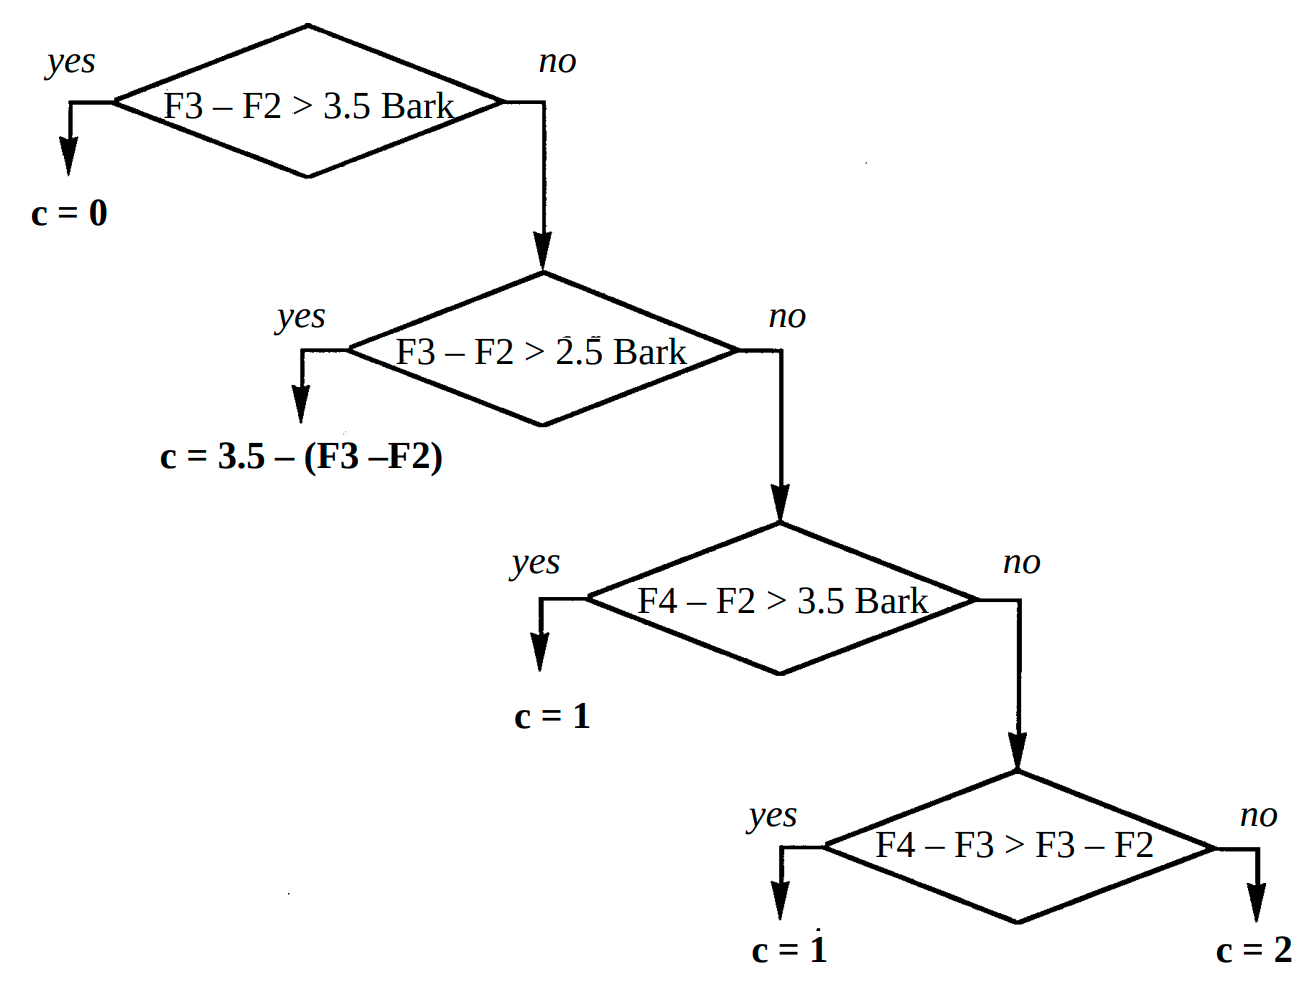
\includegraphics[width=0.5\linewidth]{images/improving/effective_second_formant.png}
    \captionsetup{width=\linewidth}
    \captionsetup{justification=centering}
    \caption{C calculation for effective second formant equation. Strategy and figure by \citet{Schwartz1997}}.
    \label{fig:effective_second_formant}
\end{figure}

\begin{equation}
  F'_2 = \frac{c_2F_2 + c_3F_3 + c_4F_4}{c_2 + c_3 + c_4}
    \begin{cases}
      c_2 = 1, c_3 = 0, c_4 = 0 & \text{if } c = 0 \\
      c_2 = 1, c_3 = 0.5, c_4 = 0 & \text{if } 0 \leq c \leq 1 \\
      c_2 = 0, c_3 = 1, c_4 = 0.5 & \text{else}
    \end{cases} 
\label{eq:effective_second_formant}      
\end{equation}

%------------------------------------

\section{Reachable acoustic space}
\label{sec:reachable_acoustic_space}

To visualise the impact of the change \texttt{Bark Operator} the reachable acoustic space was approximated by plotting multiple points.
This experiment is visualised in Figure \ref{fig:acoustic_reach}.
The alternative implementation visually differs in multiple ways.
As computer scientists, we find the more continuous nature of the implementation by \citet{deBoer2000} more pleasing.
However, an expert should ideally determine which of the two is more realistic.
In Chapter \ref{ch:results} it is discussed that the results of the experiment remain similar independent of the used variant.

\begin{figure*}[ht]
    \centering
    \begin{subfigure}{.45\textwidth}
        \centering
        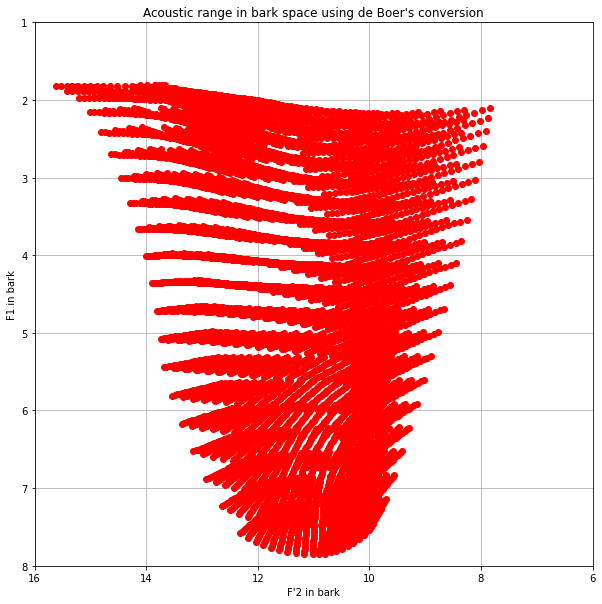
\includegraphics[width=\textwidth]{images/improving/reachable_acoustic_space-de_boer.png}
        \captionsetup{width=0.9\linewidth}
        \captionsetup{justification=centering}
        \caption{Default implementation}
    \end{subfigure}
    \hspace{0.5cm}
    \begin{subfigure}{.45\textwidth}
        \centering
        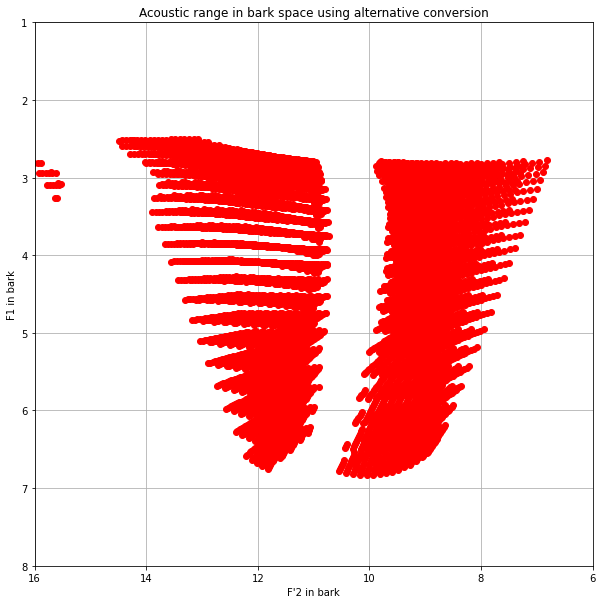
\includegraphics[width=\textwidth]{images/improving/reachable_acoustic_space-alternative.png}
        \captionsetup{width=0.9\linewidth}
        \captionsetup{justification=centering}
        \caption{Alternative implementation}
    \end{subfigure}
    \captionsetup{width=0.8\linewidth}
    \captionsetup{justification=centering}
    \caption{Reachable acoustic space of both Bark Operator alternatives.}
    \label{fig:acoustic_reach}
\end{figure*}
\chapter{Testing emergence for a small community}
\label{ch:extension}

In the previous chapter we addressed some \textit{ad hoc} design decisions made by \citet{deBoer2000}.
In this chapter we present another extension on the original model by \citet{deBoer2000}.
Instead of using random selection for initiator and imitator pairs, we use a small-community-like network.
This network is based on 5 main groups of agents, each with different influence on each other.
The network can behave both vertical as horizontal, i.e. generational or not.
This extension is a demonstration on how the provided code can be used to easily configure new experiments.


%------------------------------------

\section{Small-community-like network}
\label{sec:network_idea}

\begin{figure}[H]
    \centering
    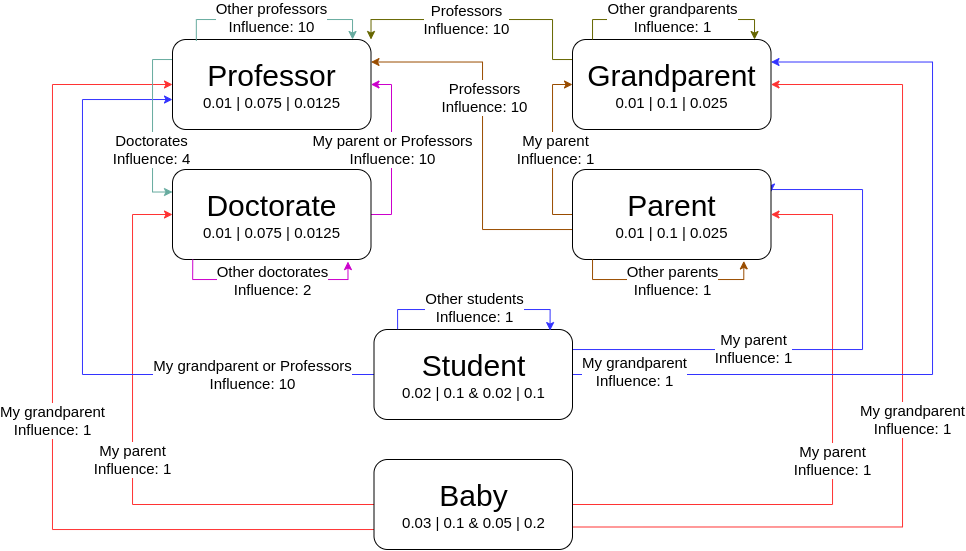
\includegraphics[width=\linewidth]{images/extension/network.png}
    \captionsetup{width=\linewidth}
    \captionsetup{justification=centering}
    \caption{Properties of small community network used.\\Arrows indicate an influential role for the agent accompanied by its weight.\\Notation underneath role: new sound probability $|$ ambient noise $|$ phoneme step size.}
    \label{fig:network}
\end{figure}
\chapter{Results}
\label{ch:results}

As discussed during in the re-implementation chapter, some of the design decisions by \citet{deBoer2000} were rather ad hoc.


%------------------------------------

\section{TODO}
\label{sec:results_XXX}

TODO
\chapter{Discussion}
\label{ch:discussion}

TODO

%------------------------------------

\section{TODO}
\label{sec:discussion_XXX}

TODO
\chapter*{Extra figures}
\label{ch:extra_figures}
\addcontentsline{toc}{chapter}{Extra figures}

To make the report more readable some figures are not provided directly in the text.
These figures are provided here.
We like to remind you that all of the figures from this report and many more can be found on the GitHub repository of this project \citep{github_project}.

\section*{Effect of decreasing phoneme step size}
\begin{figure*}[ht]
    \centering
    \begin{subfigure}{.45\textwidth}
        \centering
        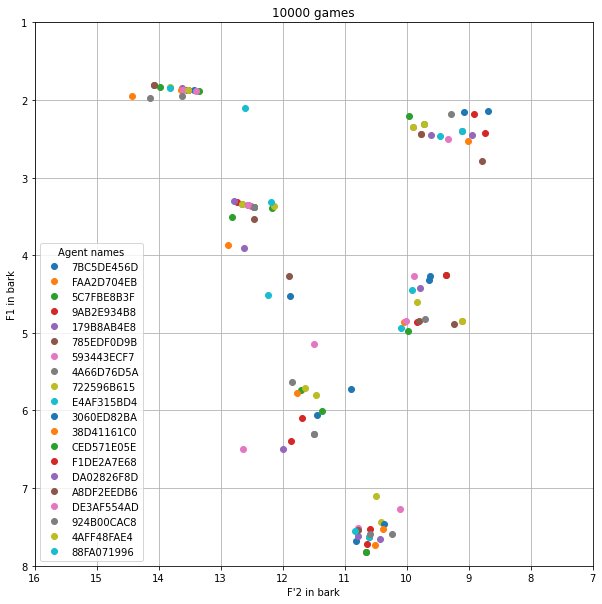
\includegraphics[width=\textwidth]{images/results/step_size_1.png}
        \captionsetup{width=0.9\linewidth}
        \captionsetup{justification=centering}
        \caption{Phoneme step size 0.1}
    \end{subfigure}
    \hspace{0.5cm}
    \begin{subfigure}{.45\textwidth}
        \centering
        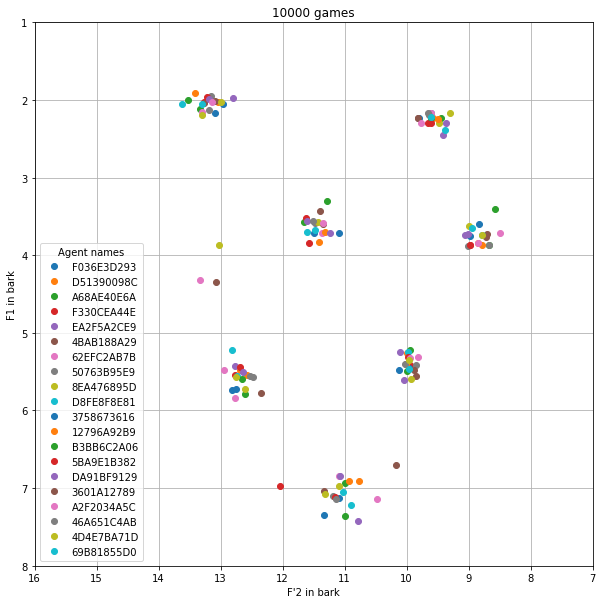
\includegraphics[width=\textwidth]{images/results/step_size_025.png}
        \captionsetup{width=0.9\linewidth}
        \captionsetup{justification=centering}
        \caption{Phoneme step size 0.025}
    \end{subfigure}
    \captionsetup{width=0.8\linewidth}
    \captionsetup{justification=centering}
    \caption{Vowel system emerged from two simulation using differing phoneme step size.}
    \label{fig:bdb_smaller_step}
\end{figure*}

\clearpage
\section*{Varying acoustic noise parameter settings for alternative bark operator}
\begin{figure*}[ht]
    \centering
    \begin{subfigure}{.30\textwidth}
        \centering
        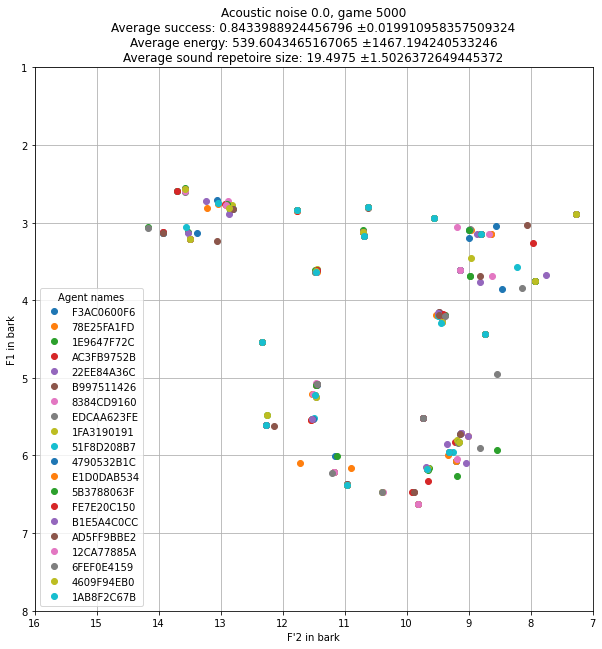
\includegraphics[width=\textwidth]{images/extra/bark_noise_1.png}
        \captionsetup{width=0.9\linewidth}
        \captionsetup{justification=centering}
        \caption{Acoustic noise = 0}
    \end{subfigure}
    \hspace{0.5cm}
    \begin{subfigure}{.30\textwidth}
        \centering
        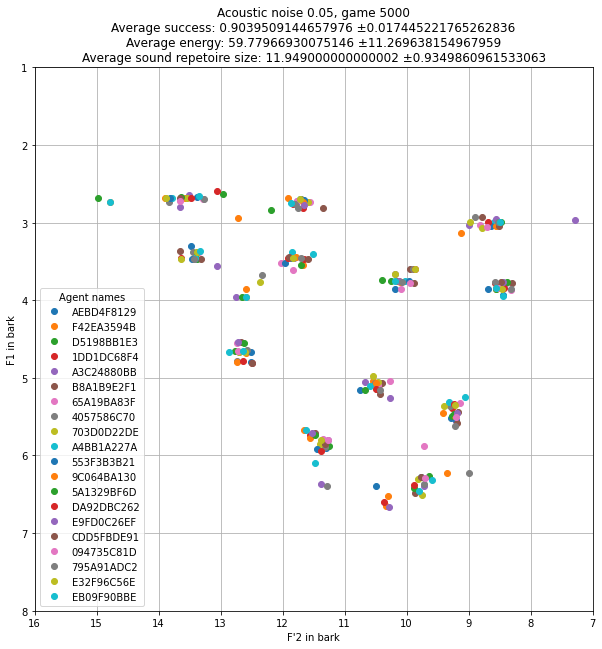
\includegraphics[width=\textwidth]{images/extra/bark_noise_2.png}
        \captionsetup{width=0.9\linewidth}
        \captionsetup{justification=centering}
        \caption{Acoustic noise = 0.05}
    \end{subfigure}
    \hspace{0.5cm}
    \begin{subfigure}{.30\textwidth}
        \centering
        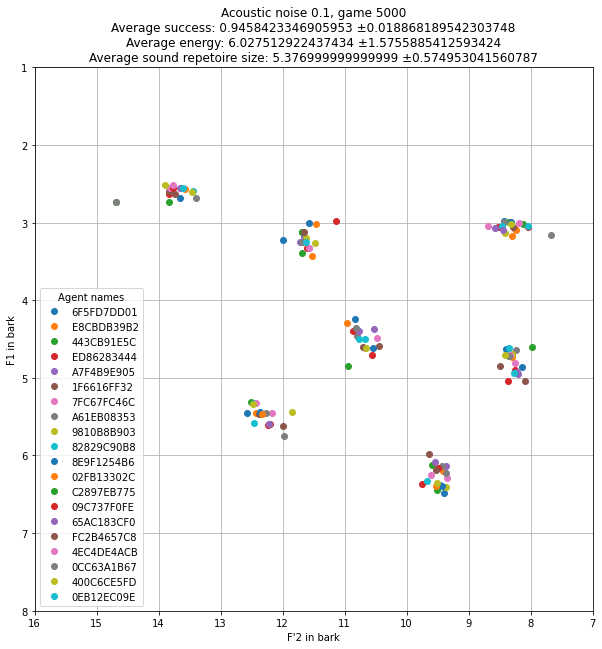
\includegraphics[width=\textwidth]{images/extra/bark_noise_3.png}
        \captionsetup{width=0.9\linewidth}
        \captionsetup{justification=centering}
        \caption{Acoustic noise = 0.1}
    \end{subfigure}
    \begin{subfigure}{.30\textwidth}
        \centering
        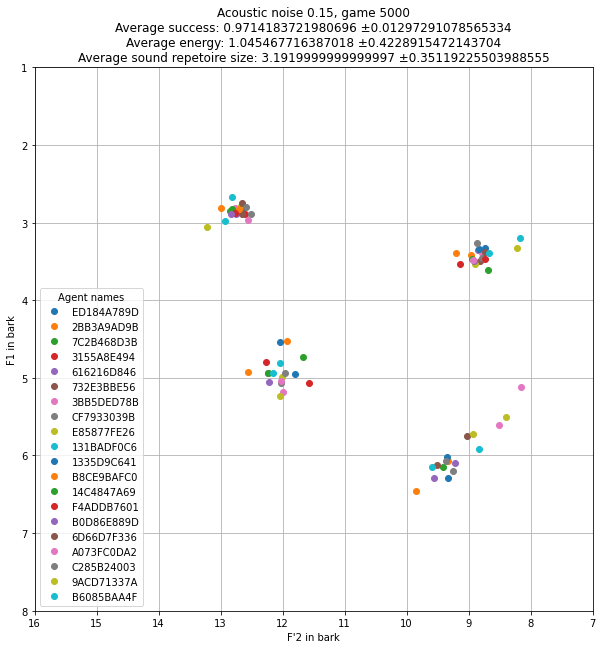
\includegraphics[width=\textwidth]{images/extra/bark_noise_4.png}
        \captionsetup{width=0.9\linewidth}
        \captionsetup{justification=centering}
        \caption{Acoustic noise = 0.15}
    \end{subfigure}
    \hspace{0.5cm}
    \begin{subfigure}{.30\textwidth}
        \centering
        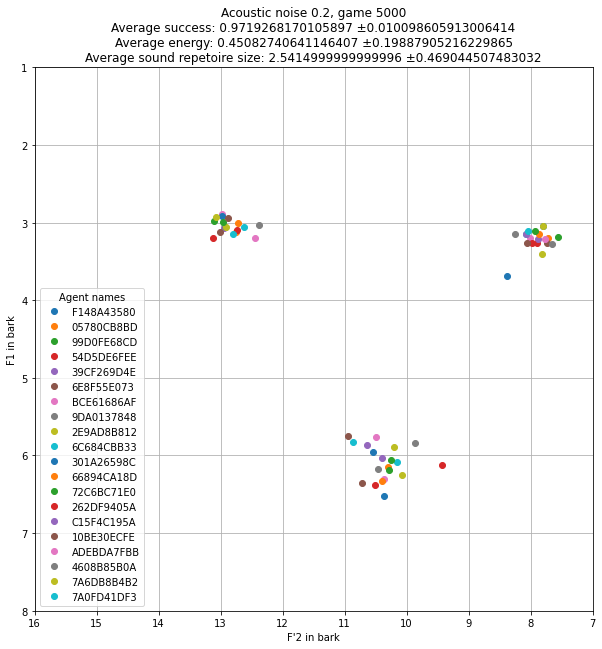
\includegraphics[width=\textwidth]{images/extra/bark_noise_5.png}
        \captionsetup{width=0.9\linewidth}
        \captionsetup{justification=centering}
        \caption{Acoustic noise = 0.2}
    \end{subfigure}
    \hspace{0.5cm}
    \begin{subfigure}{.30\textwidth}
        \centering
        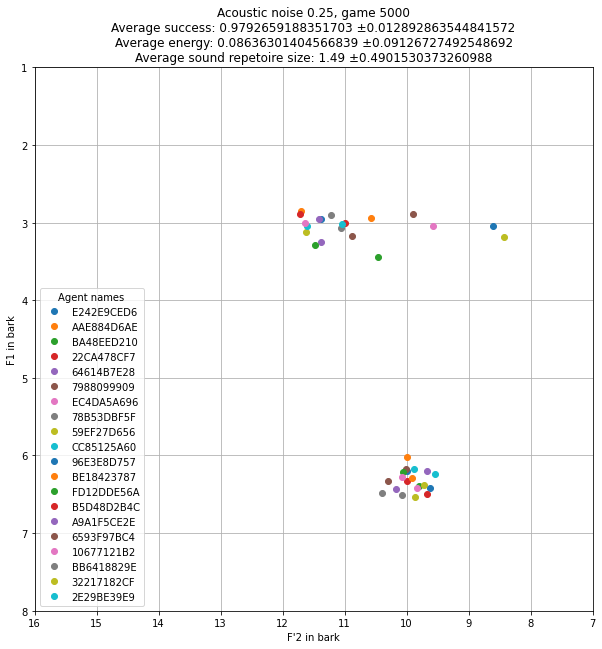
\includegraphics[width=\textwidth]{images/extra/bark_noise_6.png}
        \captionsetup{width=0.9\linewidth}
        \captionsetup{justification=centering}
        \caption{Acoustic noise = 0.25}
    \end{subfigure}
    \captionsetup{width=0.9\linewidth}
    \captionsetup{justification=centering}
    \caption{Sample games of ABM using alternative bark operator for varying acoustic noise parameters. Statistical measures are provided above each plot.}
    \label{fig:bark_noise_impact}
\end{figure*}

\clearpage
\section*{Varying effective second formant weight for alternative bark operator}
\begin{figure*}[ht]
    \centering
    \begin{subfigure}{.30\textwidth}
        \centering
        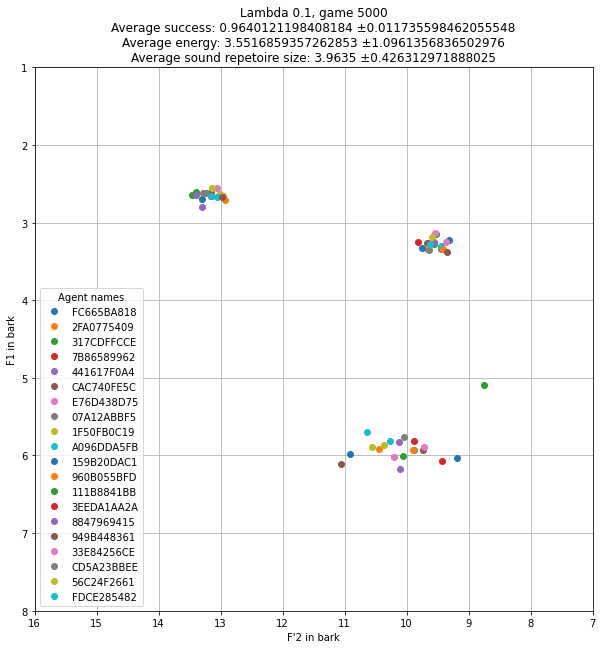
\includegraphics[width=\textwidth]{images/extra/bark_weight_1.png}
        \captionsetup{width=0.9\linewidth}
        \captionsetup{justification=centering}
        \caption{Weight = 0.1}
    \end{subfigure}
    \hspace{0.5cm}
    \begin{subfigure}{.30\textwidth}
        \centering
        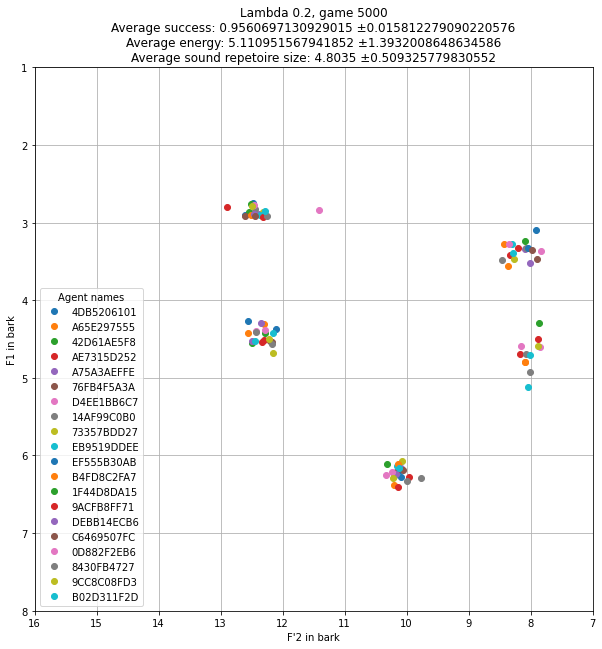
\includegraphics[width=\textwidth]{images/extra/bark_weight_2.png}
        \captionsetup{width=0.9\linewidth}
        \captionsetup{justification=centering}
        \caption{Weight = 0.2}
    \end{subfigure}
    \hspace{0.5cm}
    \begin{subfigure}{.30\textwidth}
        \centering
        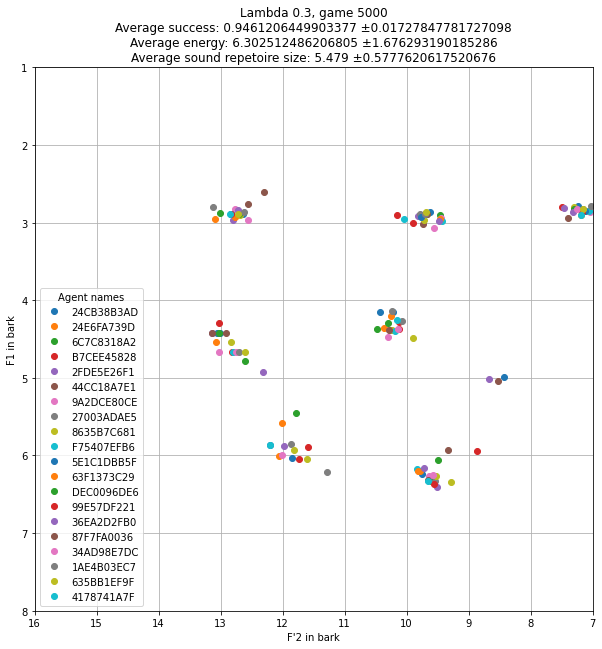
\includegraphics[width=\textwidth]{images/extra/bark_weight_3.png}
        \captionsetup{width=0.9\linewidth}
        \captionsetup{justification=centering}
        \caption{Weight = 0.3}
    \end{subfigure}
    \begin{subfigure}{.30\textwidth}
        \centering
        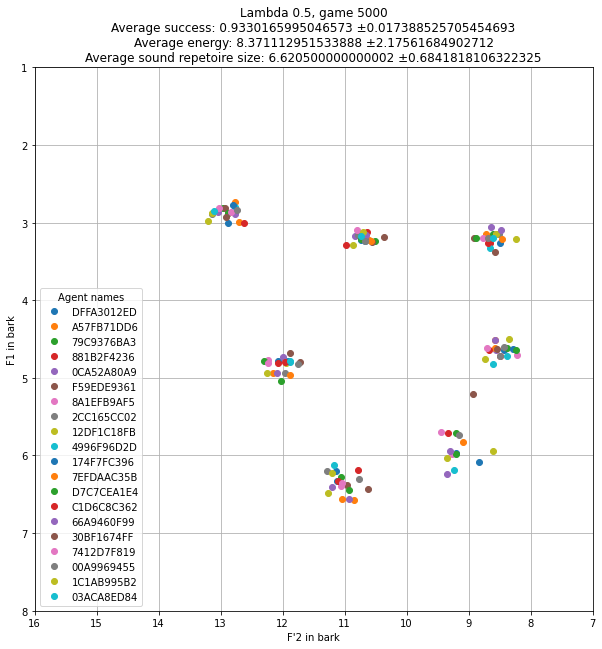
\includegraphics[width=\textwidth]{images/extra/bark_weight_4.png}
        \captionsetup{width=0.9\linewidth}
        \captionsetup{justification=centering}
        \caption{Weight = 0.5}
    \end{subfigure}
    \hspace{0.5cm}
    \begin{subfigure}{.30\textwidth}
        \centering
        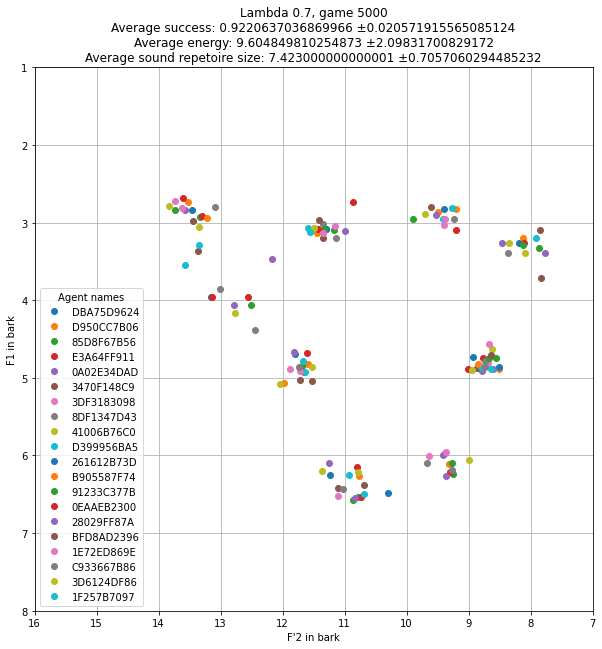
\includegraphics[width=\textwidth]{images/extra/bark_weight_5.png}
        \captionsetup{width=0.9\linewidth}
        \captionsetup{justification=centering}
        \caption{Weight = 0.7}
    \end{subfigure}
    \hspace{0.5cm}
    \begin{subfigure}{.30\textwidth}
        \centering
        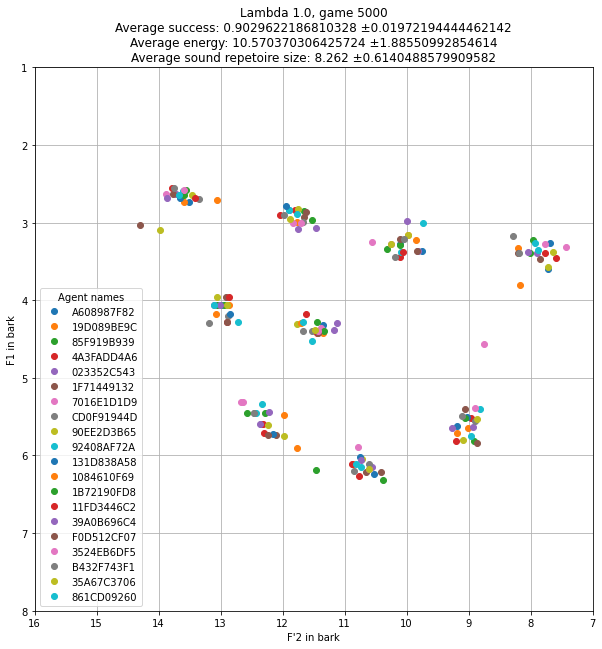
\includegraphics[width=\textwidth]{images/extra/bark_weight_6.png}
        \captionsetup{width=0.9\linewidth}
        \captionsetup{justification=centering}
        \caption{Weight = 1.0}
    \end{subfigure}
    \captionsetup{width=0.9\linewidth}
    \captionsetup{justification=centering}
    \caption{Sample games of ABM using alternative bark operator for varying effective second formant weights. Statistical measures are provided above each plot.}
    \label{fig:bark_weight_impact}
\end{figure*}

\clearpage
\section*{Overlay of known vowels}
\begin{figure}[ht]
    \centering
    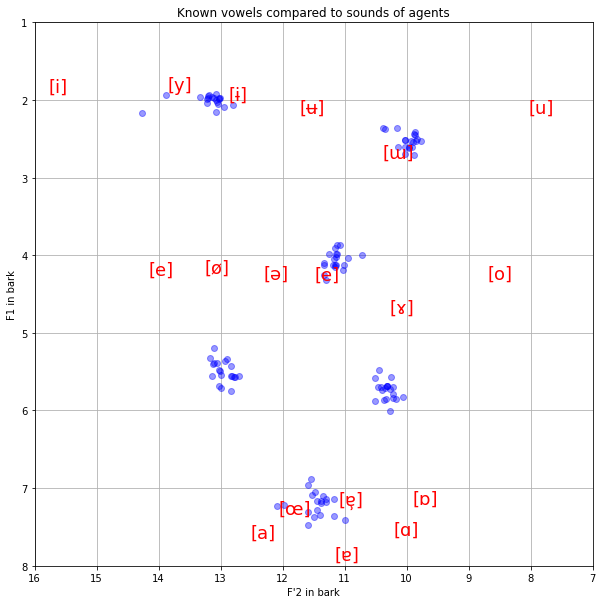
\includegraphics[width=0.6\linewidth]{images/results/overlayed_known_sounds.png}
    \captionsetup{width=\linewidth}
    \captionsetup{justification=centering}
    \caption{Overlay of known vowels on the result of a 5000 iteration imitation game.}
    \label{fig:overlayed_vowel}
\end{figure}


%references list
\nocite{*}
\printbibliography[heading=bibintoc, title={References}]
\end{document}
